% !TEX program = xelatex
\documentclass[11pt,a4paper]{article}

\usepackage[UTF8]{ctex}
\usepackage[margin=2.2cm]{geometry}
\usepackage{amsmath, amssymb, amsthm}
\usepackage{listings}
\usepackage{xcolor}
\usepackage{tikz}
\usepackage{booktabs}
\usepackage{multirow}
\usepackage{hyperref}
\usetikzlibrary{positioning, arrows.meta, shapes.geometric, fit, calc, decorations.pathreplacing}

\hypersetup{
  colorlinks=true,
  linkcolor=blue!60!black,
  urlcolor=teal!70!black,
}

\lstdefinelanguage{Rust}{
  morekeywords={fn,let,mut,pub,struct,impl,use,mod,self,Self,Option,Some,None,return,if,else,for,while,loop,match,break,continue,as,where,trait,type,enum,move,ref,const,static,unsafe,extern,crate,super,dyn,async,await,box,in},
  sensitive=true,
  morecomment=[l]{//},
  morecomment=[s]{/*}{*/},
  morestring=[b]",
}

\lstset{
  language=Rust,
  basicstyle=\ttfamily\footnotesize,
  keywordstyle=\color{blue!60!black}\bfseries,
  commentstyle=\color{green!40!black}\itshape,
  stringstyle=\color{red!60!black},
  numbers=left,
  numberstyle=\tiny\color{gray},
  numbersep=8pt,
  frame=single,
  framerule=0.4pt,
  rulecolor=\color{gray!40},
  breaklines=true,
  breakatwhitespace=true,
  showstringspaces=false,
  tabsize=4,
  columns=fullflexible,
  keepspaces=true,
}

\title{\textbf{halfedge\,: 细分模块设计文档（Loop）} \\ \large \texttt{src/subdiv.rs}（含 \texttt{catmull\_clark}、\texttt{sqrt3} 子模块）}
\author{halfedge 库}
\date{2026-07-04}

\begin{document}
\maketitle
\tableofcontents

\section{模块定位}

\texttt{subdiv.rs} 在 \texttt{traversal.rs}、\texttt{io.rs} 之上叠加
\textbf{曲面细分}能力，是 halfedge 库的细分入口。本文件直接实现 \textbf{Loop 细分}，
并通过两个子模块提供另外两种细分方案：

\begin{itemize}
  \item \texttt{subdiv::catmull\_clark}：Catmull-Clark 细分（任意多边形输入，
        输出三角化的四边形网格），详见 \texttt{docs/catmull\_clark.tex}；
  \item \texttt{subdiv::sqrt3}：√3 细分（三角网格，面数 $3\times$ 增长），
        详见 \texttt{docs/sqrt3.tex}。
\end{itemize}

Loop 细分灵感来自 OpenMesh 和 CGAL，用于三角网格的光滑细分。

\subsection{核心 API}

\begin{center}
\begin{tabular}{@{}ll@{}}
  \toprule
  \textbf{API} & \textbf{语义} \\
  \midrule
  \texttt{loop\_subdivide(\&mesh) -> MeshStorage} & 对三角网格执行一次 Loop 细分，返回新网格 \\
  \texttt{catmull\_clark\_subdivide(\&mesh)} & Catmull-Clark 细分（见 \texttt{catmull\_clark} 子模块） \\
  \texttt{sqrt3\_subdivide(\&mesh)} & √3 细分（见 \texttt{sqrt3} 子模块） \\
  \bottomrule
\end{tabular}
\end{center}

\subsection{依赖关系}

\begin{center}
\begin{tabular}{@{}ll@{}}
  \toprule
  \textbf{依赖模块} & \textbf{用途} \\
  \midrule
  \texttt{storage} & \texttt{MeshStorage} 容器、\texttt{Vertex}/\texttt{HalfEdge}/\texttt{Face} \\
  \texttt{traversal} & \texttt{VertexRing}、\texttt{FaceHalfEdges}、\texttt{is\_boundary\_*} \\
  \texttt{io} & \texttt{build\_mesh\_from\_vertices\_and\_faces} 构建新网格 \\
  \bottomrule
\end{tabular}
\end{center}

\section{算法概述}

Loop 细分是一种\textbf{逼近型}细分方案，每次细分将每个三角面分裂为 4 个小
三角形，同时按加权平均更新所有顶点位置，使网格趋于光滑。

\subsection{规模变化}

设原始网格有 $V$ 顶点、$E$ 边、$F$ 面，细分后：
\[
  V' = V + E, \quad F' = 4F, \quad E' = 4E
\]

\textbf{验证}（以 \texttt{icosphere(1)} 为例）：
\begin{center}
\begin{tabular}{@{}lccccc@{}}
  \toprule
   & $V$ & $E$ & $F$ & $V{-}E{+}F$ & 说明 \\
  \midrule
  细分前 & 42  & 120 & 80  & 2 & icosphere(1) \\
  细分后 & 162 & 480 & 320 & 2 & $V{+}E{=}162$，$4F{=}320$ \\
  \bottomrule
\end{tabular}
\end{center}

Euler 示性数 $V - E + F = 2$ 在细分过程中保持不变（闭合三角网格）。

\subsection{算法流程图}

\begin{center}
\begin{tikzpicture}[
  node distance=0.5cm and 0.8cm,
  box/.style={draw, rounded corners=2pt, minimum width=3.6cm, minimum height=0.8cm, align=center, font=\footnotesize},
  arrow/.style={-Stealth, thick, draw=blue!60!black}
]
  \node[box, fill=blue!10] (input) {输入 \texttt{\&MeshStorage}};
  \node[box, fill=yellow!20, below=of input] (collect) {收集顶点 ID / 面索引\\建立 \texttt{VertexId $\to$ u32} 映射};
  \node[box, fill=green!15, below=of collect] (edge) {遍历半边\\计算每条边的中点位置};
  \node[box, fill=green!15, below=of edge] (vert) {遍历原始顶点\\计算更新后的位置};
  \node[box, fill=orange!20, below=of vert] (split) {每个三角面分裂为 4 个};
  \node[box, fill=blue!10, below=of split] (build) {\texttt{build\_mesh\_from\_vertices\_and\_faces}};
  \node[box, fill=red!10, below=of build] (output) {输出新 \texttt{MeshStorage}};

  \draw[arrow] (input) -- (collect);
  \draw[arrow] (collect) -- (edge);
  \draw[arrow] (edge) -- (vert);
  \draw[arrow] (vert) -- (split);
  \draw[arrow] (split) -- (build);
  \draw[arrow] (build) -- (output);
\end{tikzpicture}
\end{center}

\section{边点计算}

\subsection{公式}

对每条边 $(v_0, v_1)$，根据是否为边界边采用不同权重：

\textbf{内部边}（两侧都有面）：
\[
  v_{\text{new}} = \frac{3}{8}(v_0 + v_1) + \frac{1}{8}(v_2 + v_3)
\]
其中 $v_2, v_3$ 是该边两侧相对顶点：
\begin{itemize}
  \item $v_2 = \texttt{he.next.vertex}$（\texttt{he} 所在面的对边顶点）
  \item $v_3 = \texttt{twin.next.vertex}$（\texttt{twin} 所在面的对边顶点）
\end{itemize}

\textbf{边界边}（至少一侧无面）：
\[
  v_{\text{new}} = \frac{1}{2}(v_0 + v_1)
\]

\subsection{几何图示}

\begin{center}
\begin{tikzpicture}[
  vert/.style={circle, draw=blue!70!black, fill=blue!10, minimum size=6mm, inner sep=0pt, font=\small},
  newv/.style={circle, draw=red!70!black, fill=red!10, minimum size=6mm, inner sep=0pt, font=\small},
  edge/.style={thick, draw=gray!70!black},
  newe/.style={thick, draw=red!70!black, dashed}
]
  % 内部边情况
  \node[vert] (v0) at (0,0) {$v_0$};
  \node[vert] (v1) at (4,0) {$v_1$};
  \node[vert] (v2) at (2,1.8) {$v_2$};
  \node[vert] (v3) at (2,-1.8) {$v_3$};
  \node[newv] (m) at (2,0) {$v_{\text{new}}$};

  \draw[edge] (v0) -- (v2);
  \draw[edge] (v1) -- (v2);
  \draw[edge] (v0) -- (v3);
  \draw[edge] (v1) -- (v3);
  \draw[newe] (v0) -- (v1);

  \node[font=\footnotesize, right=0.1cm of m] {$= \frac{3}{8}(v_0{+}v_1) + \frac{1}{8}(v_2{+}v_3)$};

  \node[font=\scriptsize, gray, below=1.6cm of m, align=center]
    {内部边：两侧相对顶点 $v_2, v_3$ 共同贡献 $\frac{1}{8}$ 权重};
\end{tikzpicture}
\end{center}

\subsection{实现要点}

\begin{itemize}
  \item 用 \texttt{HashMap<(u32, u32), u32>} 缓存每条无向边的中点索引，
        键为 $\bigl(\min(i_0, i_1), \max(i_0, i_1)\bigr)$，保证每条边只处理一次；
  \item 遍历所有半边（含边界半边），用 \texttt{is\_boundary\_edge} 判定边类型；
  \item 内部边若拓扑不完整（\texttt{next} 或 \texttt{twin.next} 缺失），
        退化为边界边公式（防御性处理）。
\end{itemize}

\section{顶点更新}

\subsection{内部顶点}

设顶点 $v$ 的 valence 为 $n$（邻居数），则更新公式：
\[
  v' = (1 - n\beta)\, v + \beta \sum_{i=1}^{n} v_i
\]
其中 $\beta$ 由 Loop 给出：
\[
  \beta = \frac{1}{n}\left[\frac{5}{8} - \left(\frac{3}{8} + \frac{1}{4}\cos\frac{2\pi}{n}\right)^{\!2}\right]
\]

\textbf{正则情况}（$n = 6$）：
\[
  \cos\frac{2\pi}{6} = \frac{1}{2}, \quad
  \frac{3}{8} + \frac{1}{4}\cdot\frac{1}{2} = \frac{1}{2}, \quad
  \beta = \frac{1}{6}\left(\frac{5}{8} - \frac{1}{4}\right) = \frac{1}{16}
\]
\[
  v' = \frac{5}{8}v + \frac{1}{16}\sum_{i=1}^{6} v_i
\]

\textbf{非正则情况}（$n = 3$）：
\[
  \cos\frac{2\pi}{3} = -\frac{1}{2}, \quad
  \beta = \frac{1}{3}\left[\frac{5}{8} - \left(\frac{1}{4}\right)^{\!2}\right] = \frac{3}{16}
\]

\subsection{边界顶点}

边界顶点 $v$ 沿边界方向有两个邻居 $v_{\text{prev}}, v_{\text{next}}$，更新公式：
\[
  v' = \frac{1}{8}v_{\text{prev}} + \frac{3}{4}v + \frac{1}{8}v_{\text{next}}
\]

\subsection{邻居识别}

\textbf{内部顶点}：通过 \texttt{VertexRing::new(mesh, v)} 遍历所有 outgoing
半边，每条半边的 \texttt{vertex}（tip）即一个邻居。

\textbf{边界顶点}：同样遍历 outgoing 半边，但用 \texttt{is\_boundary\_edge}
过滤，得到恰好 2 个边界邻居。

\section{面分裂}

每个原始三角形 $(a, b, c)$ 在三条边中点处插入新顶点 $ab, bc, ca$，
分裂为 4 个小三角形：
\[
  (a, b, c) \;\longrightarrow\;
  \begin{cases}
    (a, ab, ca) \\
    (b, bc, ab) \\
    (c, ca, bc) \\
    (ab, bc, ca)
  \end{cases}
\]

\begin{center}
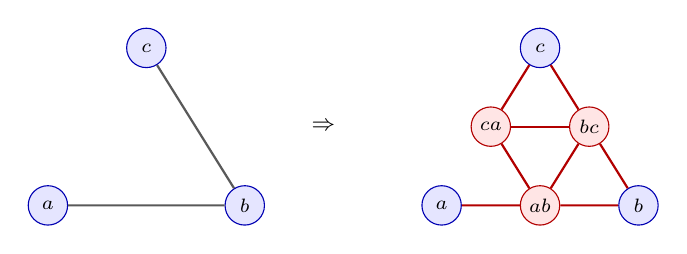
\begin{tikzpicture}[
  vert/.style={circle, draw=blue!70!black, fill=blue!10, minimum size=5mm, inner sep=0pt, font=\scriptsize},
  newv/.style={circle, draw=red!70!black, fill=red!10, minimum size=5mm, inner sep=0pt, font=\scriptsize},
  edge/.style={thick, draw=gray!70!black},
  newe/.style={thick, draw=red!70!black}
]
  % 原始三角形
  \node[vert] (a1) at (0,0) {$a$};
  \node[vert] (b1) at (2.5,0) {$b$};
  \node[vert] (c1) at (1.25,2) {$c$};
  \draw[edge] (a1) -- (b1) -- (c1) -- cycle;

  \node[font=\footnotesize] at (3.5,1) {$\Rightarrow$};

  % 细分后
  \node[vert] (a2) at (5,0) {$a$};
  \node[vert] (b2) at (7.5,0) {$b$};
  \node[vert] (c2) at (6.25,2) {$c$};
  \node[newv] (ab) at (6.25,0) {$ab$};
  \node[newv] (bc) at (6.875,1) {$bc$};
  \node[newv] (ca) at (5.625,1) {$ca$};

  \draw[newe] (a2) -- (ab) -- (b2) -- (bc) -- (c2) -- (ca) -- cycle;
  \draw[newe] (ab) -- (ca);
  \draw[newe] (ab) -- (bc);
  \draw[newe] (bc) -- (ca);
\end{tikzpicture}
\end{center}

\section{同步更新}

Loop 细分要求\textbf{同步更新}：所有新位置（边中点 + 原始顶点更新）
都基于\textbf{旧位置}计算，最后一次性应用。

本实现的策略：
\begin{enumerate}
  \item \texttt{new\_positions} 初始填充原始顶点的旧位置；
  \item 步骤 3 计算边中点时，\texttt{new\_positions[0..V]} 仍为旧值，直接读取；
  \item 步骤 4 计算原始顶点新位置时，从 \texttt{mesh} 读取旧位置（\texttt{mesh} 全程不修改），
        结果暂存到独立 \texttt{updated\_orig} 向量；
  \item 步骤 4 末尾将 \texttt{updated\_orig} 覆盖回 \texttt{new\_positions[0..V]}。
\end{enumerate}

\section{实现代码}

\subsection{核心函数签名}

\begin{lstlisting}
pub fn loop_subdivide(mesh: &MeshStorage) -> MeshStorage
\end{lstlisting}

\subsection{边点计算}

\begin{lstlisting}
let midpoint = if is_boundary_edge(mesh, he_id) {
    // 边界边：1/2*(v0+v1)
    [
        0.5 * (p0[0] + p1[0]),
        0.5 * (p0[1] + p1[1]),
        0.5 * (p0[2] + p1[2]),
    ]
} else {
    // 内部边：3/8*(v0+v1) + 1/8*(v2+v3)
    let v2 = h.next.and_then(|n| mesh.get_halfedge(n)).map(|n| n.vertex);
    let v3 = h.twin.and_then(|t| mesh.get_halfedge(t))
                .and_then(|t| t.next)
                .and_then(|n| mesh.get_halfedge(n))
                .map(|n| n.vertex);
    // ...
};
\end{lstlisting}

\subsection{$\beta$ 权重}

\begin{lstlisting}
fn loop_beta(n: usize) -> f64 {
    if n == 0 { return 0.0; }  // 守卫：除零
    let n_f = n as f64;
    let cos_term = (2.0 * std::f64::consts::PI / n_f).cos();
    let inner = 3.0/8.0 + 1.0/4.0 * cos_term;
    (1.0 / n_f) * (5.0/8.0 - inner * inner)
}
\end{lstlisting}

\section{健壮性}

\begin{itemize}
  \item \textbf{无效 / 已删除 ID}：所有查询通过 \texttt{mesh.get\_*} + \texttt{Option}
        链式调用，\texttt{None} 时跳过该边 / 该顶点；
  \item \textbf{边界顶点邻居数 $\neq 2$}：保持原位置（退化情况）；
  \item \textbf{内部顶点 valence $= 0$}：保持原位置（孤立顶点）；
  \item \textbf{内部边拓扑不完整}（\texttt{next} / \texttt{twin.next} 缺失）：
        退化为边界边公式；
  \item \texttt{loop\_beta(0)} 守卫除零，返回 $0$；
  \item \textbf{空网格}：返回空网格，不 panic；
  \item \textbf{非三角面}：Loop 细分仅支持三角形。若输入含非三角面
        （如四边形），这些面会被\textbf{跳过}并通过 \texttt{eprintln!}
        输出警告到 stderr，含跳过面数与替代建议（\texttt{catmull\_clark\_subdivide}）。
        三角面照常细分。详见 \texttt{loop\_subdivide\_skips\_non\_triangle\_with\_warning}
        与 \texttt{loop\_subdivide\_mixed\_mesh\_keeps\_only\_triangles} 测试。
\end{itemize}

\section{复杂度分析}

设原始网格有 $V$ 顶点、$E$ 边、$F$ 面。

\begin{center}
\renewcommand{\arraystretch}{1.20}
\begin{tabular}{@{}lll@{}}
  \toprule
  \textbf{步骤} & \textbf{时间} & \textbf{空间} \\
  \midrule
  收集顶点 / 面索引     & $O(V + F)$       & $O(V + F)$ \\
  边点计算（每条边一次） & $O(E)$           & $O(E)$（中点缓存） \\
  顶点更新（每个顶点遍历邻居） & $O(V + E)$ & $O(V)$（新位置数组） \\
  面分裂                & $O(F)$           & $O(F)$（新面数组） \\
  构建新网格            & $O(V' + E' + F')$ & $O(V' + E' + F')$ \\
  \midrule
  \textbf{总计}         & $O(V + E + F)$   & $O(V' + E' + F')$ \\
  \bottomrule
\end{tabular}
\end{center}

其中 $V' = V + E$，$E' = 4E$，$F' = 4F$。

\section{测试覆盖}

\begin{center}
\renewcommand{\arraystretch}{1.18}
\begin{tabular}{@{}ll@{}}
  \toprule
  \textbf{测试名} & \textbf{验证内容} \\
  \midrule
  \texttt{loop\_subdivide\_icosphere1\_vertex\_face\_count} & icosphere(1) 细分后 V=162, F=320 \\
  \texttt{loop\_subdivide\_icosphere0\_vertex\_face\_count} & icosphere(0) 细分后 V=42, F=80 \\
  \texttt{loop\_subdivide\_icosphere2\_vertex\_face\_count} & icosphere(2) 细分后 V=642, F=1280 \\
  \texttt{loop\_subdivide\_passes\_topology\_validation}   & 细分后通过 \texttt{check\_topology} \\
  \texttt{loop\_subdivide\_icosphere2\_passes\_validation} & icosphere(2) 细分后通过校验 \\
  \texttt{loop\_subdivide\_preserves\_euler\_characteristic} & Euler 示性数 $V{-}E{+}F{=}2$ 保持 \\
  \texttt{loop\_subdivide\_single\_triangle}               & 单三角面片细分后 V=6, F=4 \\
  \texttt{loop\_subdivide\_open\_quad}                     & 开四边形细分后 V=9, F=8 \\
  \texttt{loop\_subdivide\_boundary\_edge\_midpoint}       & 边界边中点位置 $= \frac{1}{2}(v_0{+}v_1)$ \\
  \texttt{loop\_subdivide\_interior\_edge\_midpoint}       & 内部边中点位置 $= \frac{3}{8}(v_0{+}v_1) + \frac{1}{8}(v_2{+}v_3)$ \\
  \texttt{loop\_beta\_regular\_valence\_6}                 & $\beta(6) = \frac{1}{16}$ \\
  \texttt{loop\_beta\_valence\_3}                          & $\beta(3) = \frac{3}{16}$ \\
  \texttt{loop\_beta\_zero\_valence\_returns\_zero}        & $\beta(0) = 0$（不 panic） \\
  \texttt{loop\_subdivide\_multiple\_iterations\_stay\_valid} & 连续 3 次细分拓扑校验通过 \\
  \texttt{loop\_subdivide\_empty\_mesh}                    & 空网格细分返回空网格 \\
  \midrule
  \texttt{loop\_subdivide\_skips\_non\_triangle\_with\_warning} & 单四边形面输入：跳过，输出 0 面（stderr 警告） \\
  \texttt{loop\_subdivide\_mixed\_mesh\_keeps\_only\_triangles} & 三角形 + 四边形混合输入：仅三角形细分为 4 面 \\
  \bottomrule
\end{tabular}
\end{center}

共 17 个单元测试，全部通过。\texttt{cargo test} 全模块共 498 个用例，0 失败 / 0 警告。
细分模块（含 \texttt{catmull\_clark} 11 个与 \texttt{sqrt3} 16 个子模块测试）合计 44 个测试。

\section{示例输出}

\texttt{cargo run --example loop\_subdivision} 的关键输出：

\begin{lstlisting}[basicstyle=\ttfamily\scriptsize, numbers=none, frame=single]
[1] 单次 Loop 细分规模变化
  细分前 icosphere(1): V=   42 F=   80 E=  120 HE=  240
  细分后              : V=  162 F=  320 E=  480 HE=  960
  规模验证：V'=V+E (42+120=162)，F'=4F (4*80=320)
  拓扑校验：OK

[3] 细分后顶点度数分布（icosphere(0) → 细分 1 次）
  度数 5 的顶点数 = 12
  度数 6 的顶点数 = 30
  （icosphere(0) 的 12 个原始顶点度数=5，细分后仍保持度数=5；
   新增的边中点度数=6，符合 Loop 细分的正则性质）

[4] Euler 示性数 V - E + F 保持不变
  细分 0x: V-E+F = 12-30+20 = 2（应为 2）
  细分 1x: V-E+F = 42-120+80 = 2（应为 2）
  细分 2x: V-E+F = 162-480+320 = 2（应为 2）
  细分 3x: V-E+F = 642-1920+1280 = 2（应为 2）
\end{lstlisting}

\section{设计取舍}

\begin{itemize}
  \item \textbf{为何复用 \texttt{build\_mesh\_from\_vertices\_and\_faces}？}
        该函数已经处理了 twin / next / prev / 边界环 / 顶点入口 / 面入口
        的完整构建，避免在本模块重复实现半边拓扑构造逻辑。
  \item \textbf{为何用 \texttt{HashMap} 缓存边中点？}
        每条无向边只需计算一次中点。用 $(\min, \max)$ 键去重，
        保证 $O(E)$ 时间 / $O(E)$ 空间。
  \item \textbf{为何同步更新而非渐进更新？}
        Loop 细分要求所有新位置基于旧位置计算。若渐进修改，
        后续顶点会读到已更新的邻居位置，破坏算法正确性。
        本实现用独立 \texttt{updated\_orig} 向量暂存，最后统一覆盖。
  \item \textbf{为何边界顶点邻居数 $\neq 2$ 时保持原位置？}
        正常流形网格的边界顶点恰好有 2 个边界邻居。邻居数 $\neq 2$
        说明拓扑非流形或退化，此时不应用边界公式，保持原位置是安全降级。
  \item \textbf{为何不投影回球面？}
        Loop 细分是\textbf{逼近型}细分，不保留原始曲面。
        \texttt{test\_util} 中 icosphere 生成器的细分
        会把新顶点投影回球面，那是 icosphere 的特殊行为，
        不是 Loop 细分本身的职责。
\end{itemize}

\end{document}
